The classification task was to properly delineate between images with severe retinopathy present and images with no retinopathy. The model was asses based on its loss metrics and the AUC-ROC score over 50 epochs.

In \autoref{fig:lossEpoch}, we show the model's training and validation loss over 50 epochs. It demonstrates with increasing epochs the training loss consistently decreased while the validation loss reached its minimum value after about 10 epochs, then continued to increase. This suggests the model will proceed to overfit on the data after roughly 10 epochs.

\begin{figure*}[t]
  \centering
  \begin{minipage}{.5\textwidth}
    \centering
    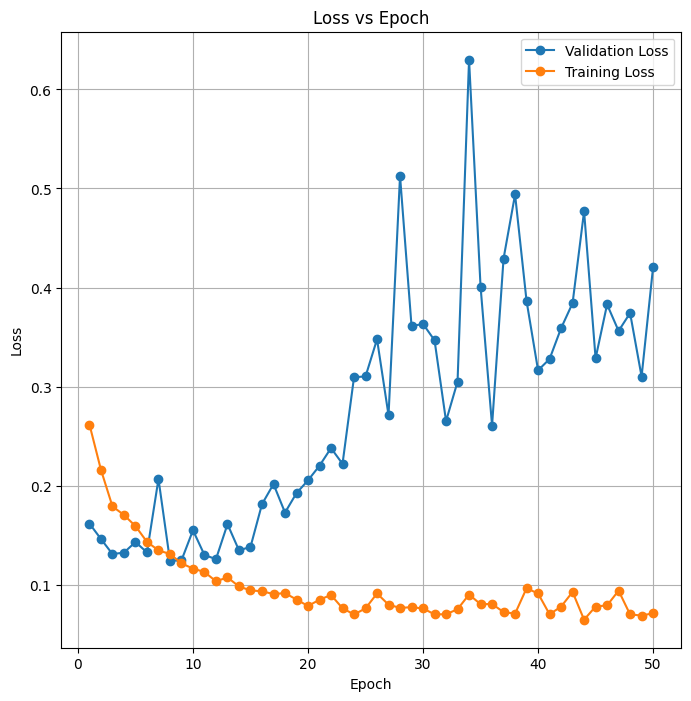
\includegraphics[scale=0.35]{Images/lossEpoch.png}
    \caption{Model loss per epoch}
    \label{fig:lossEpoch}
  \end{minipage}%
  \begin{minipage}{.5\textwidth}
    \centering
    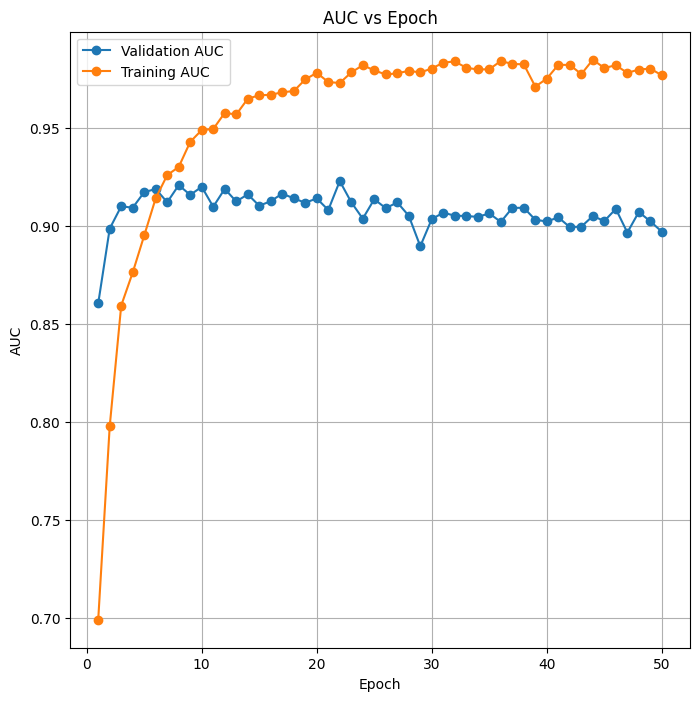
\includegraphics[scale=0.35]{Images/aucEpoch.png}
    \caption{Model AUC-ROC score per epoch}
    \label{fig:auc-roc}
  \end{minipage}
\end{figure*}

The training and validation AUC-ROC scores, as depicted in \autoref{fig:auc-roc}, demonstrate a rapid initial increase within just a few epochs of training. Specifically, the training AUC-ROC score shows a continuous upward trend throughout the 50 epochs, reaching a peak of approximately 0.98. In contrast, the validation AUC-ROC score attains its maximum value of around 0.92 by the 10th epoch, after which it exhibits a modest decline, indicating potential overfitting to the training data. Consequently, we have decided to adopt the model parameters corresponding to the epoch where the validation accuracy peaked.

The VGG16 model demonstrated strong performance in the binary classification of diabetic retinopathy images, achieving a peak validation AUC-ROC score of 0.92. This suggests a 92\% probability that the model can accurately differentiate between the two classes, indicating a high level of separability. Consequently, we consider the model to be successful in performing the binary classification task.

\autoref{fig:epochtime} illustrates the comparative training times for each epoch between two computing environments: GPU and CPU. The graph clearly shows that the model trained on the NVIDIA T4 GPU, which leverages a parallel architecture, was significantly more time-efficient. On average, the GPU completed an epoch in just 6 minutes and 28 seconds, whereas the CPU took 2 hours, 50 minutes, and 5 seconds to finish an epoch. This stark contrast highlights that the GPU was approximately 26 times faster than the CPU for each training epoch.
\begin{figure}[!ht]
    \centering
    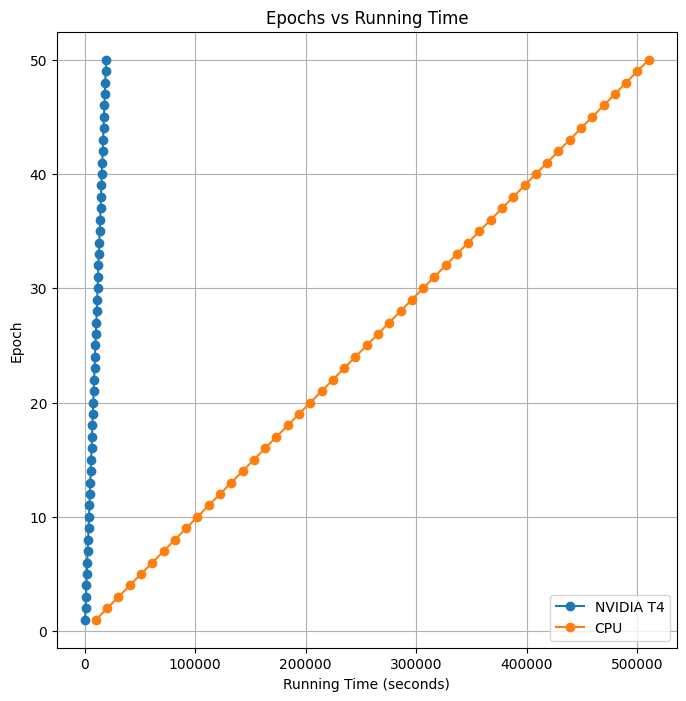
\includegraphics[scale=0.35]{Images/runningTime.png}
    \caption{Number of epochs completed over time}
    \label{fig:epochtime}
\end{figure}